% Digital Logic Report Template
% Created: 2020-01-10, John Miller

%==========================================================
%=========== Document Setup  ==============================

% Formatting defined by class file
\documentclass[11pt]{article}

% ---- Document formatting ----
\usepackage[margin=1in]{geometry}	% Narrower margins
\usepackage{booktabs}				% Nice formatting of tables
\usepackage{graphicx}				% Ability to include graphics

%\setlength\parindent{0pt}	% Do not indent first line of paragraphs 
\usepackage[parfill]{parskip}		% Line space b/w paragraphs
%	parfill option prevents last line of pgrph from being fully justified

% Parskip package adds too much space around titles, fix with this
\RequirePackage{titlesec}
\titlespacing\section{0pt}{8pt plus 4pt minus 2pt}{3pt plus 2pt minus 2pt}
\titlespacing\subsection{0pt}{4pt plus 4pt minus 2pt}{-2pt plus 2pt minus 2pt}
\titlespacing\subsubsection{0pt}{2pt plus 4pt minus 2pt}{-6pt plus 2pt minus 2pt}

% ---- Hyperlinks ----
\usepackage[colorlinks=true,urlcolor=blue]{hyperref}	% For URL's. Automatically links internal references.

% ---- Code listings ----
\usepackage{listings} 					% Nice code layout and inclusion
\usepackage[usenames,dvipsnames]{xcolor}	% Colors (needs to be defined before using colors)

% Define custom colors for listings
\definecolor{listinggray}{gray}{0.98}		% Listings background color
\definecolor{rulegray}{gray}{0.7}			% Listings rule/frame color

% Style for Verilog
\lstdefinestyle{Verilog}{
	language=Verilog,					% Verilog
	backgroundcolor=\color{listinggray},	% light gray background
	rulecolor=\color{blue}, 			% blue frame lines
	frame=tb,							% lines above & below
	linewidth=\columnwidth, 			% set line width
	basicstyle=\small\ttfamily,	% basic font style that is used for the code	
	breaklines=true, 					% allow breaking across columns/pages
	tabsize=3,							% set tab size
	commentstyle=\color{gray},	% comments in italic 
	stringstyle=\upshape,				% strings are printed in normal font
	showspaces=false,					% don't underscore spaces
}

% How to use: \Verilog[listing_options]{file}
\newcommand{\Verilog}[2][]{%
	\lstinputlisting[style=Verilog,#1]{#2}
}




%======================================================
%=========== Body  ====================================
\begin{document}

\title{ELC 2137 Lab 0: Lab Title}
\author{Yiting Wang}

\maketitle


\section*{Summary}

Type the summary of your experiment and results here.  


\section*{Q\&A}

\begin{enumerate}
	\item List  of  errors  found  during  simulation.   What does this tell you about why we run simulations? \\
	 \\
	\item How many wires are connected to the 7-segment display?  If the segments werenotall connectedtogether,  how  many  wires  would  there  have  tobe?   Why  do  we  prefer  the  current  method  vs.separating all of the segments?\\
\end{enumerate}




\section*{Results}

	Firgure 1 is the simulation waveform and ERT of mux2_4b.\\
	\begin{figure}[ht]\centering
		\begin{tabular}{l|rrrr}
			Time (ns): & 0 & 10 & 20 & 30 \\
			\midrule
			in1 & 1111 & 1111 & 0100 & 0100 \\
			in0 & 0000 & 0000 & 1101 & 1101 \\
			sel & 0 & 1 & 0 & 1 \\
			\midrule
			out & 0000 & 1111 & 1101 & 0100 \\
			\bottomrule
		\end{tabular}\medskip
		
		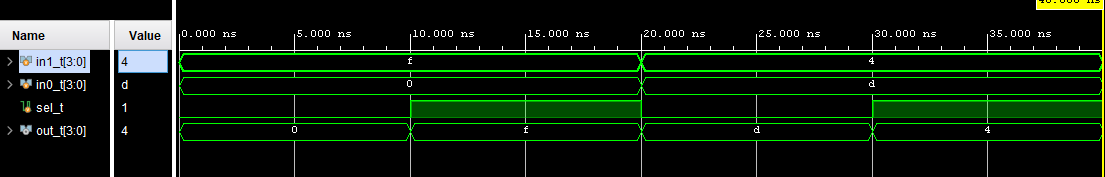
\includegraphics[width=1\textwidth]{mux2_4b_simulation}
		\caption{the simulation waveform and ERT of mux2_4b}
		\label{fig:mux2_4b_simulation}
	\end{figure}
	
	Firgure 2 is the simulation waveform and ERT of sseg_decoder. \\
	\begin{figure}[ht]\centering
		\begin{tabular}{l|rrrr|rrrr}
			Time (ns): & 0 & 10 & 20 & 30 & 40 & 50 & 60 & 70 & 80 & 90 & 100 & 110 & 120 & 130 & 140 & 150 \\
			\midrule
			num (hex) & 0 & 1 & 2 & 3 & 4 & 5 & 6 & 7 & 8 & 9 & a & b & c & d & e & f \\
			\midrule
			sseg (hex) & 40 & 79 & 24 & 30 & 19 & 12 & 02 & 78 & 00 & 18 & 08 & 03 & 46 & 21 & 06 & 0e \\
			\bottomrule
		\end{tabular}\medskip
		
		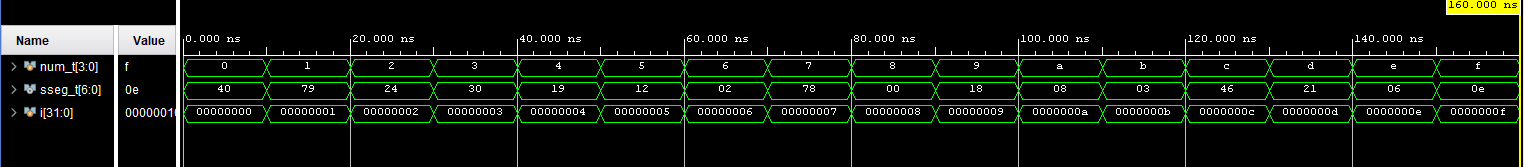
\includegraphics[width=1\textwidth]{sseg_decoder_simulation}
		\caption{the simulation waveform and ERT of sseg_decoder}
		\label{fig:sseg_decoder_simulation}
	\end{figure}
	
	Firgure 3 is the simulation waveform and ERT of sseg1. \\
	\begin{figure}[ht]\centering
		\begin{tabular}{l|rrrr|rrrr|rrrr|rr}
			Time (ns): & 0 & 10 & 20 & 30 & 40 & 50 & 60 & 70 & 80 & 90 & 100 & 110 & 120 & 130 \\
			\midrule
			A1A0 & 00 & 00 & 00 & 00 & 01 & 10 & 10 & 00 & 00 & 00 & 00 & 01 & 10 & 10 \\
			B1B0 & 00 & 01 & 10 & 11 & 01 & 01 & 00 & 00 & 01 & 10 & 11 & 01 & 01 & 00 \\
			mode & 0 & 0 & 0 & 0 & 0 & 0 & 0 & 1 & 1 & 1 & 1 & 1 & 1 & 1 \\
			\midrule
			c & 0 & 0 & 0 & 0 & 0 & 0 & 0 & 0 & 1 & 1 & 1 & 0 & 0 & 0 \\
			s1 & 0 & 0 & 1 & 1 & 1 & 1 & 1 & 0 & 1 & 1 & 0 & 0 & 0 & 1 \\
			s0 & 0 & 1 & 0 & 1 & 0 & 1 & 0 & 0 & 1 & 0 & 1 & 0 & 1 & 0 \\
			\bottomrule
		\end{tabular}\medskip
		
		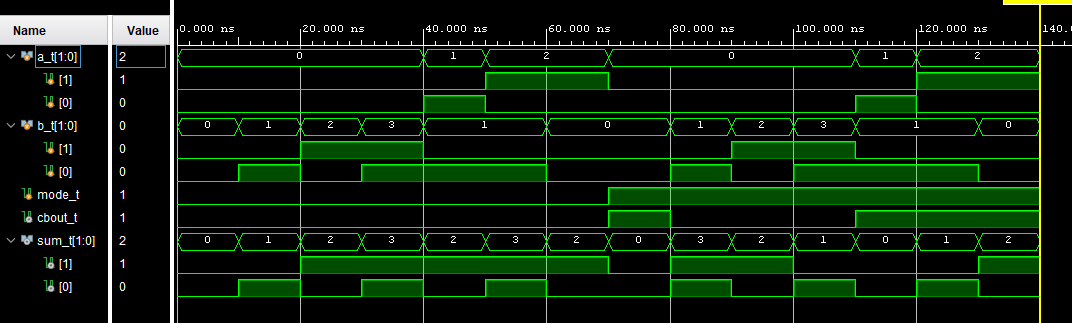
\includegraphics[width=1\textwidth]{AddSubSimulation}
		\caption{the simulation waveform and ERT of two bit adder/subtractor}
		\label{fig:AddSubSimulation}
	\end{figure}

	
	Firgure 1 is the block diagrams for half adder module. \\
	\begin{figure}[ht]\centering    
		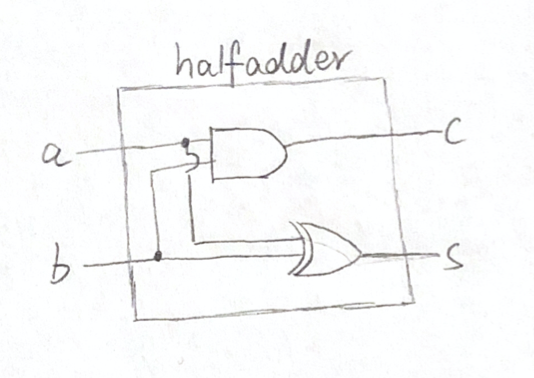
\includegraphics[width=0.5\textwidth]{halfadder}    
		\caption{This is the block diagrams for half adder module.}    
		\label{fig:halfadder}
	\end{figure}



\section*{Code}

\subsection*{File Inclusion}
\Verilog[caption=Half Adder Verilog code,label=code:file_ex]{halfadder.sv}

\subsection*{File Inclusion}
\Verilog[caption=Half Adder Test Benches Verilog code,label=code:file_ex]{halfadder_test.sv}

\subsection*{File Inclusion}
\Verilog[caption=Full Adder Verilog code,label=code:file_ex]{fulladder.sv}

\subsection*{File Inclusion}
\Verilog[caption=Full Adder Test Benches Verilog code,label=code:file_ex]{fulladder_test.sv}

\subsection*{File Inclusion}
\Verilog[caption=Two Bit Adder/Aubtractor Verilog code,label=code:file_ex]{addsub.sv}

\subsection*{File Inclusion}
\Verilog[caption=Two Bit Adder/Aubtractor Test Benches Verilog code,label=code:file_ex]{addsub_test.sv}


\end{document}
